% Options for packages loaded elsewhere
\PassOptionsToPackage{unicode}{hyperref}
\PassOptionsToPackage{hyphens}{url}
\PassOptionsToPackage{dvipsnames,svgnames,x11names}{xcolor}
%
\documentclass[
  letterpaper,
  DIV=11,
  numbers=noendperiod]{scrartcl}

\usepackage{amsmath,amssymb}
\usepackage{lmodern}
\usepackage{iftex}
\ifPDFTeX
  \usepackage[T1]{fontenc}
  \usepackage[utf8]{inputenc}
  \usepackage{textcomp} % provide euro and other symbols
\else % if luatex or xetex
  \usepackage{unicode-math}
  \defaultfontfeatures{Scale=MatchLowercase}
  \defaultfontfeatures[\rmfamily]{Ligatures=TeX,Scale=1}
\fi
% Use upquote if available, for straight quotes in verbatim environments
\IfFileExists{upquote.sty}{\usepackage{upquote}}{}
\IfFileExists{microtype.sty}{% use microtype if available
  \usepackage[]{microtype}
  \UseMicrotypeSet[protrusion]{basicmath} % disable protrusion for tt fonts
}{}
\makeatletter
\@ifundefined{KOMAClassName}{% if non-KOMA class
  \IfFileExists{parskip.sty}{%
    \usepackage{parskip}
  }{% else
    \setlength{\parindent}{0pt}
    \setlength{\parskip}{6pt plus 2pt minus 1pt}}
}{% if KOMA class
  \KOMAoptions{parskip=half}}
\makeatother
\usepackage{xcolor}
\setlength{\emergencystretch}{3em} % prevent overfull lines
\setcounter{secnumdepth}{5}
% Make \paragraph and \subparagraph free-standing
\ifx\paragraph\undefined\else
  \let\oldparagraph\paragraph
  \renewcommand{\paragraph}[1]{\oldparagraph{#1}\mbox{}}
\fi
\ifx\subparagraph\undefined\else
  \let\oldsubparagraph\subparagraph
  \renewcommand{\subparagraph}[1]{\oldsubparagraph{#1}\mbox{}}
\fi


\providecommand{\tightlist}{%
  \setlength{\itemsep}{0pt}\setlength{\parskip}{0pt}}\usepackage{longtable,booktabs,array}
\usepackage{calc} % for calculating minipage widths
% Correct order of tables after \paragraph or \subparagraph
\usepackage{etoolbox}
\makeatletter
\patchcmd\longtable{\par}{\if@noskipsec\mbox{}\fi\par}{}{}
\makeatother
% Allow footnotes in longtable head/foot
\IfFileExists{footnotehyper.sty}{\usepackage{footnotehyper}}{\usepackage{footnote}}
\makesavenoteenv{longtable}
\usepackage{graphicx}
\makeatletter
\def\maxwidth{\ifdim\Gin@nat@width>\linewidth\linewidth\else\Gin@nat@width\fi}
\def\maxheight{\ifdim\Gin@nat@height>\textheight\textheight\else\Gin@nat@height\fi}
\makeatother
% Scale images if necessary, so that they will not overflow the page
% margins by default, and it is still possible to overwrite the defaults
% using explicit options in \includegraphics[width, height, ...]{}
\setkeys{Gin}{width=\maxwidth,height=\maxheight,keepaspectratio}
% Set default figure placement to htbp
\makeatletter
\def\fps@figure{htbp}
\makeatother

\KOMAoption{captions}{tableheading}
\makeatletter
\makeatother
\makeatletter
\@ifpackageloaded{caption}{}{\usepackage{caption}}
\AtBeginDocument{%
\ifdefined\contentsname
  \renewcommand*\contentsname{Table of contents}
\else
  \newcommand\contentsname{Table of contents}
\fi
\ifdefined\listfigurename
  \renewcommand*\listfigurename{List of Figures}
\else
  \newcommand\listfigurename{List of Figures}
\fi
\ifdefined\listtablename
  \renewcommand*\listtablename{List of Tables}
\else
  \newcommand\listtablename{List of Tables}
\fi
\ifdefined\figurename
  \renewcommand*\figurename{Figure}
\else
  \newcommand\figurename{Figure}
\fi
\ifdefined\tablename
  \renewcommand*\tablename{Table}
\else
  \newcommand\tablename{Table}
\fi
}
\@ifpackageloaded{float}{}{\usepackage{float}}
\floatstyle{ruled}
\@ifundefined{c@chapter}{\newfloat{codelisting}{h}{lop}}{\newfloat{codelisting}{h}{lop}[chapter]}
\floatname{codelisting}{Listing}
\newcommand*\listoflistings{\listof{codelisting}{List of Listings}}
\makeatother
\makeatletter
\@ifpackageloaded{caption}{}{\usepackage{caption}}
\@ifpackageloaded{subcaption}{}{\usepackage{subcaption}}
\makeatother
\makeatletter
\@ifpackageloaded{tcolorbox}{}{\usepackage[many]{tcolorbox}}
\makeatother
\makeatletter
\@ifundefined{shadecolor}{\definecolor{shadecolor}{rgb}{.97, .97, .97}}
\makeatother
\makeatletter
\makeatother
\ifLuaTeX
  \usepackage{selnolig}  % disable illegal ligatures
\fi
\IfFileExists{bookmark.sty}{\usepackage{bookmark}}{\usepackage{hyperref}}
\IfFileExists{xurl.sty}{\usepackage{xurl}}{} % add URL line breaks if available
\urlstyle{same} % disable monospaced font for URLs
\hypersetup{
  pdftitle={DSS Prototype Analysis},
  pdfauthor={Alvin Murphy},
  colorlinks=true,
  linkcolor={blue},
  filecolor={Maroon},
  citecolor={Blue},
  urlcolor={Blue},
  pdfcreator={LaTeX via pandoc}}

\title{DSS Prototype Analysis}
\author{Alvin Murphy}
\date{}

\begin{document}
\maketitle
\ifdefined\Shaded\renewenvironment{Shaded}{\begin{tcolorbox}[borderline west={3pt}{0pt}{shadecolor}, sharp corners, interior hidden, frame hidden, boxrule=0pt, enhanced, breakable]}{\end{tcolorbox}}\fi

\renewcommand*\contentsname{Table of contents}
{
\hypersetup{linkcolor=}
\setcounter{tocdepth}{3}
\tableofcontents
}
\newpage

\hypertarget{dss-installation-as-a-docker-container}{%
\section{DSS Installation as a Docker
Container}\label{dss-installation-as-a-docker-container}}

https://github.com/jupyter/docker-stacks\\
https://hub.docker.com/r/jupyter/r-notebook/tags/

\emph{(optional) docker pull jupyter/r-notebook:latest}

We want the Jupyter container to mount the DDS Prototype
\textasciitilde/analysis/ directory to provide access to scripts and
data. Use the following to mount the analysis directory (i.e.~current
working directory) as a volume in the Juypter container. Note that the
directory needed to be added as a valid mount point via the Docker
Desktop Dashboard on Mac.

\emph{docker run -it --rm -d -p 10000:8888 -v
\$\{PWD\}:/home/jovyan/work --name notebook jupyter/r-notebook:latest}

To find the token from the container:\\
\emph{docker exec -it notebook jupyter server list}\\
or\\
\emph{docker logs notebook}

Navigate to the container UI and enter the token: http://localhost:10000

\hypertarget{dss-system-context}{%
\section{DSS System Context}\label{dss-system-context}}

Figure 1 depicts the context for the DSS. The DSS operator interacts
with the DSS Prototype for decision assitance. The DSS relies on a
aircraft database to gather real-time flight data to review in decision
support algorithms.

\begin{figure}

{\centering 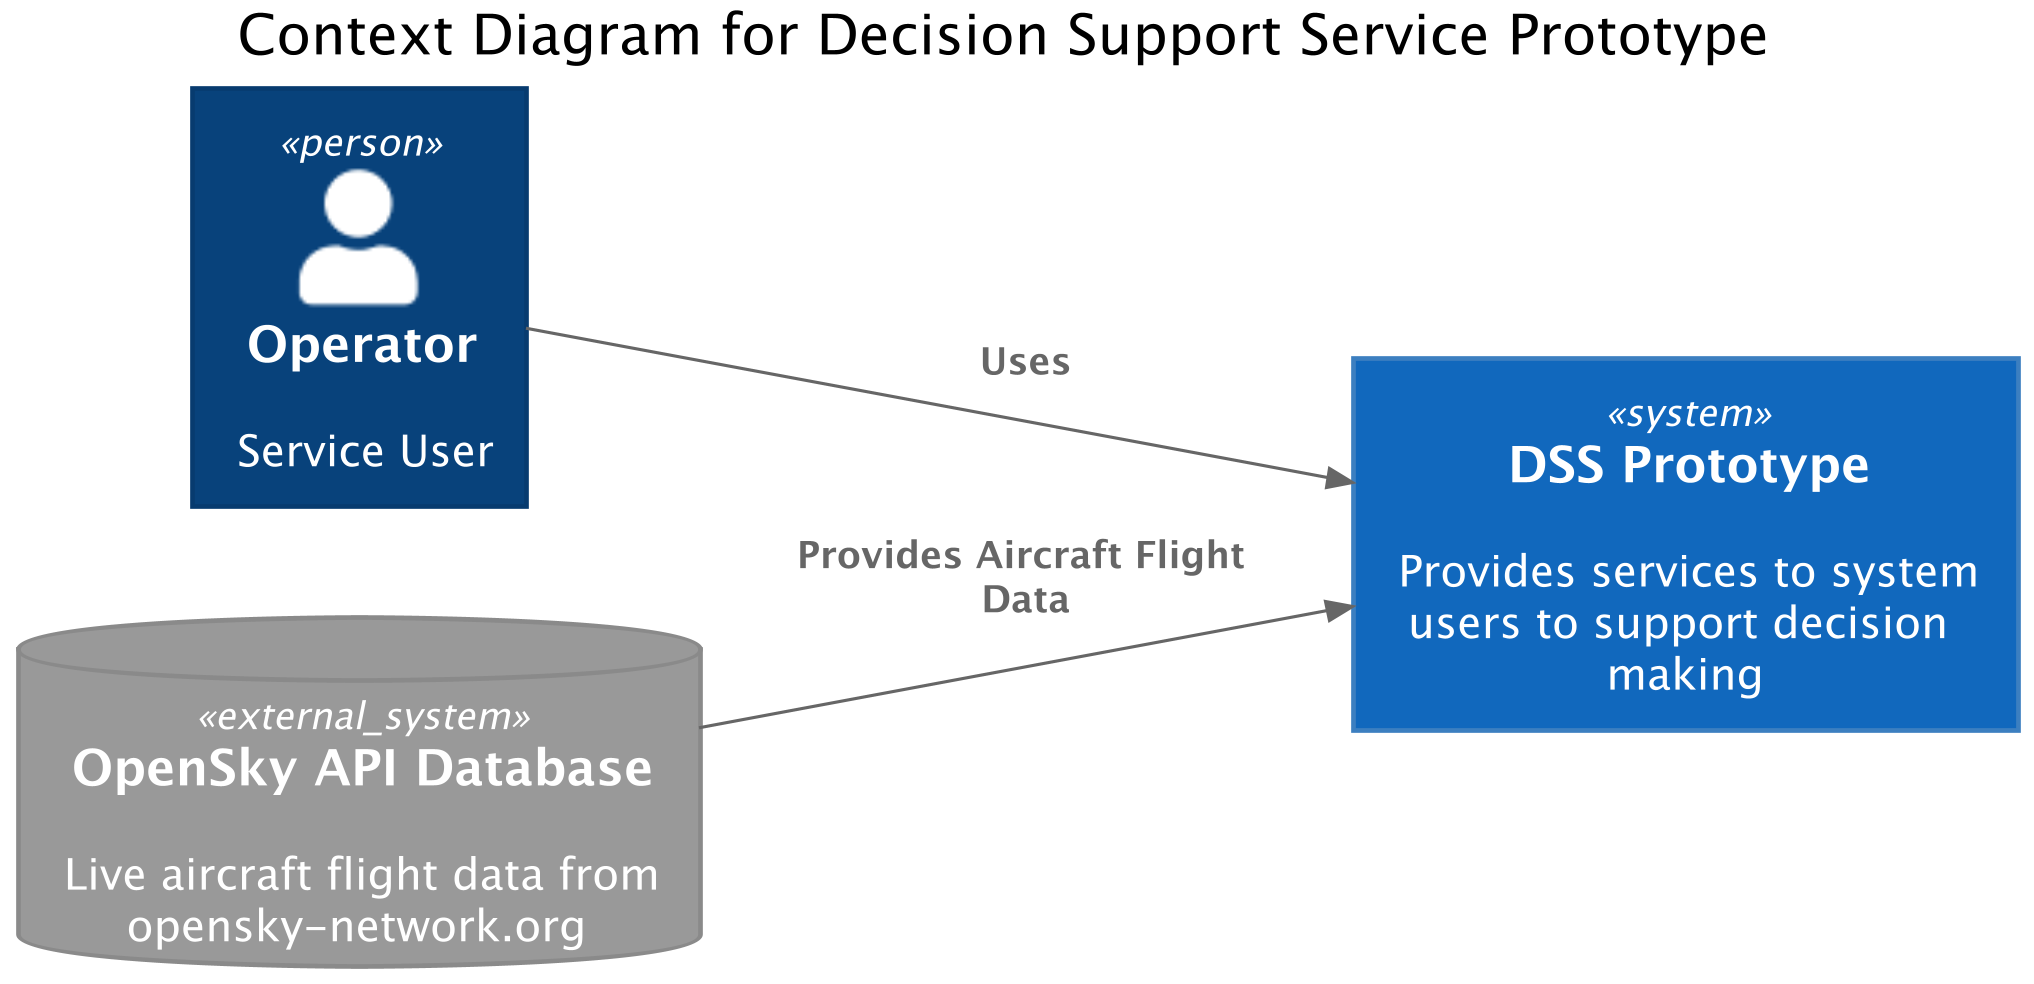
\includegraphics{dss-span-analysis-rev1_files/figure-pdf/53b3b0c0-d3c0-4526-9cfe-f74946c31414.png}

}

\caption{DSS Context Diagram}

\end{figure}

\hypertarget{dss-container-architecture}{%
\subsection{DSS Container
Architecture}\label{dss-container-architecture}}

Nine containers are instantiated as part of the DSS architecuture (see
Figure 2). Six provide the DSS implementation while the additional 3
support collection and calculation of metrics. Each application
container was designed around the 12-Factor Application ``Single
Responsibility Principle''; e.g.~each app has one purpose to enable
rapid insertion of new capabilities with low cohesion to other
functionality. At this time, all responses are canned without underlying
calculations to focus on meeting the 500 ms hypothesis pryor to
burdening the application with calculation latency.

\begin{figure}

{\centering 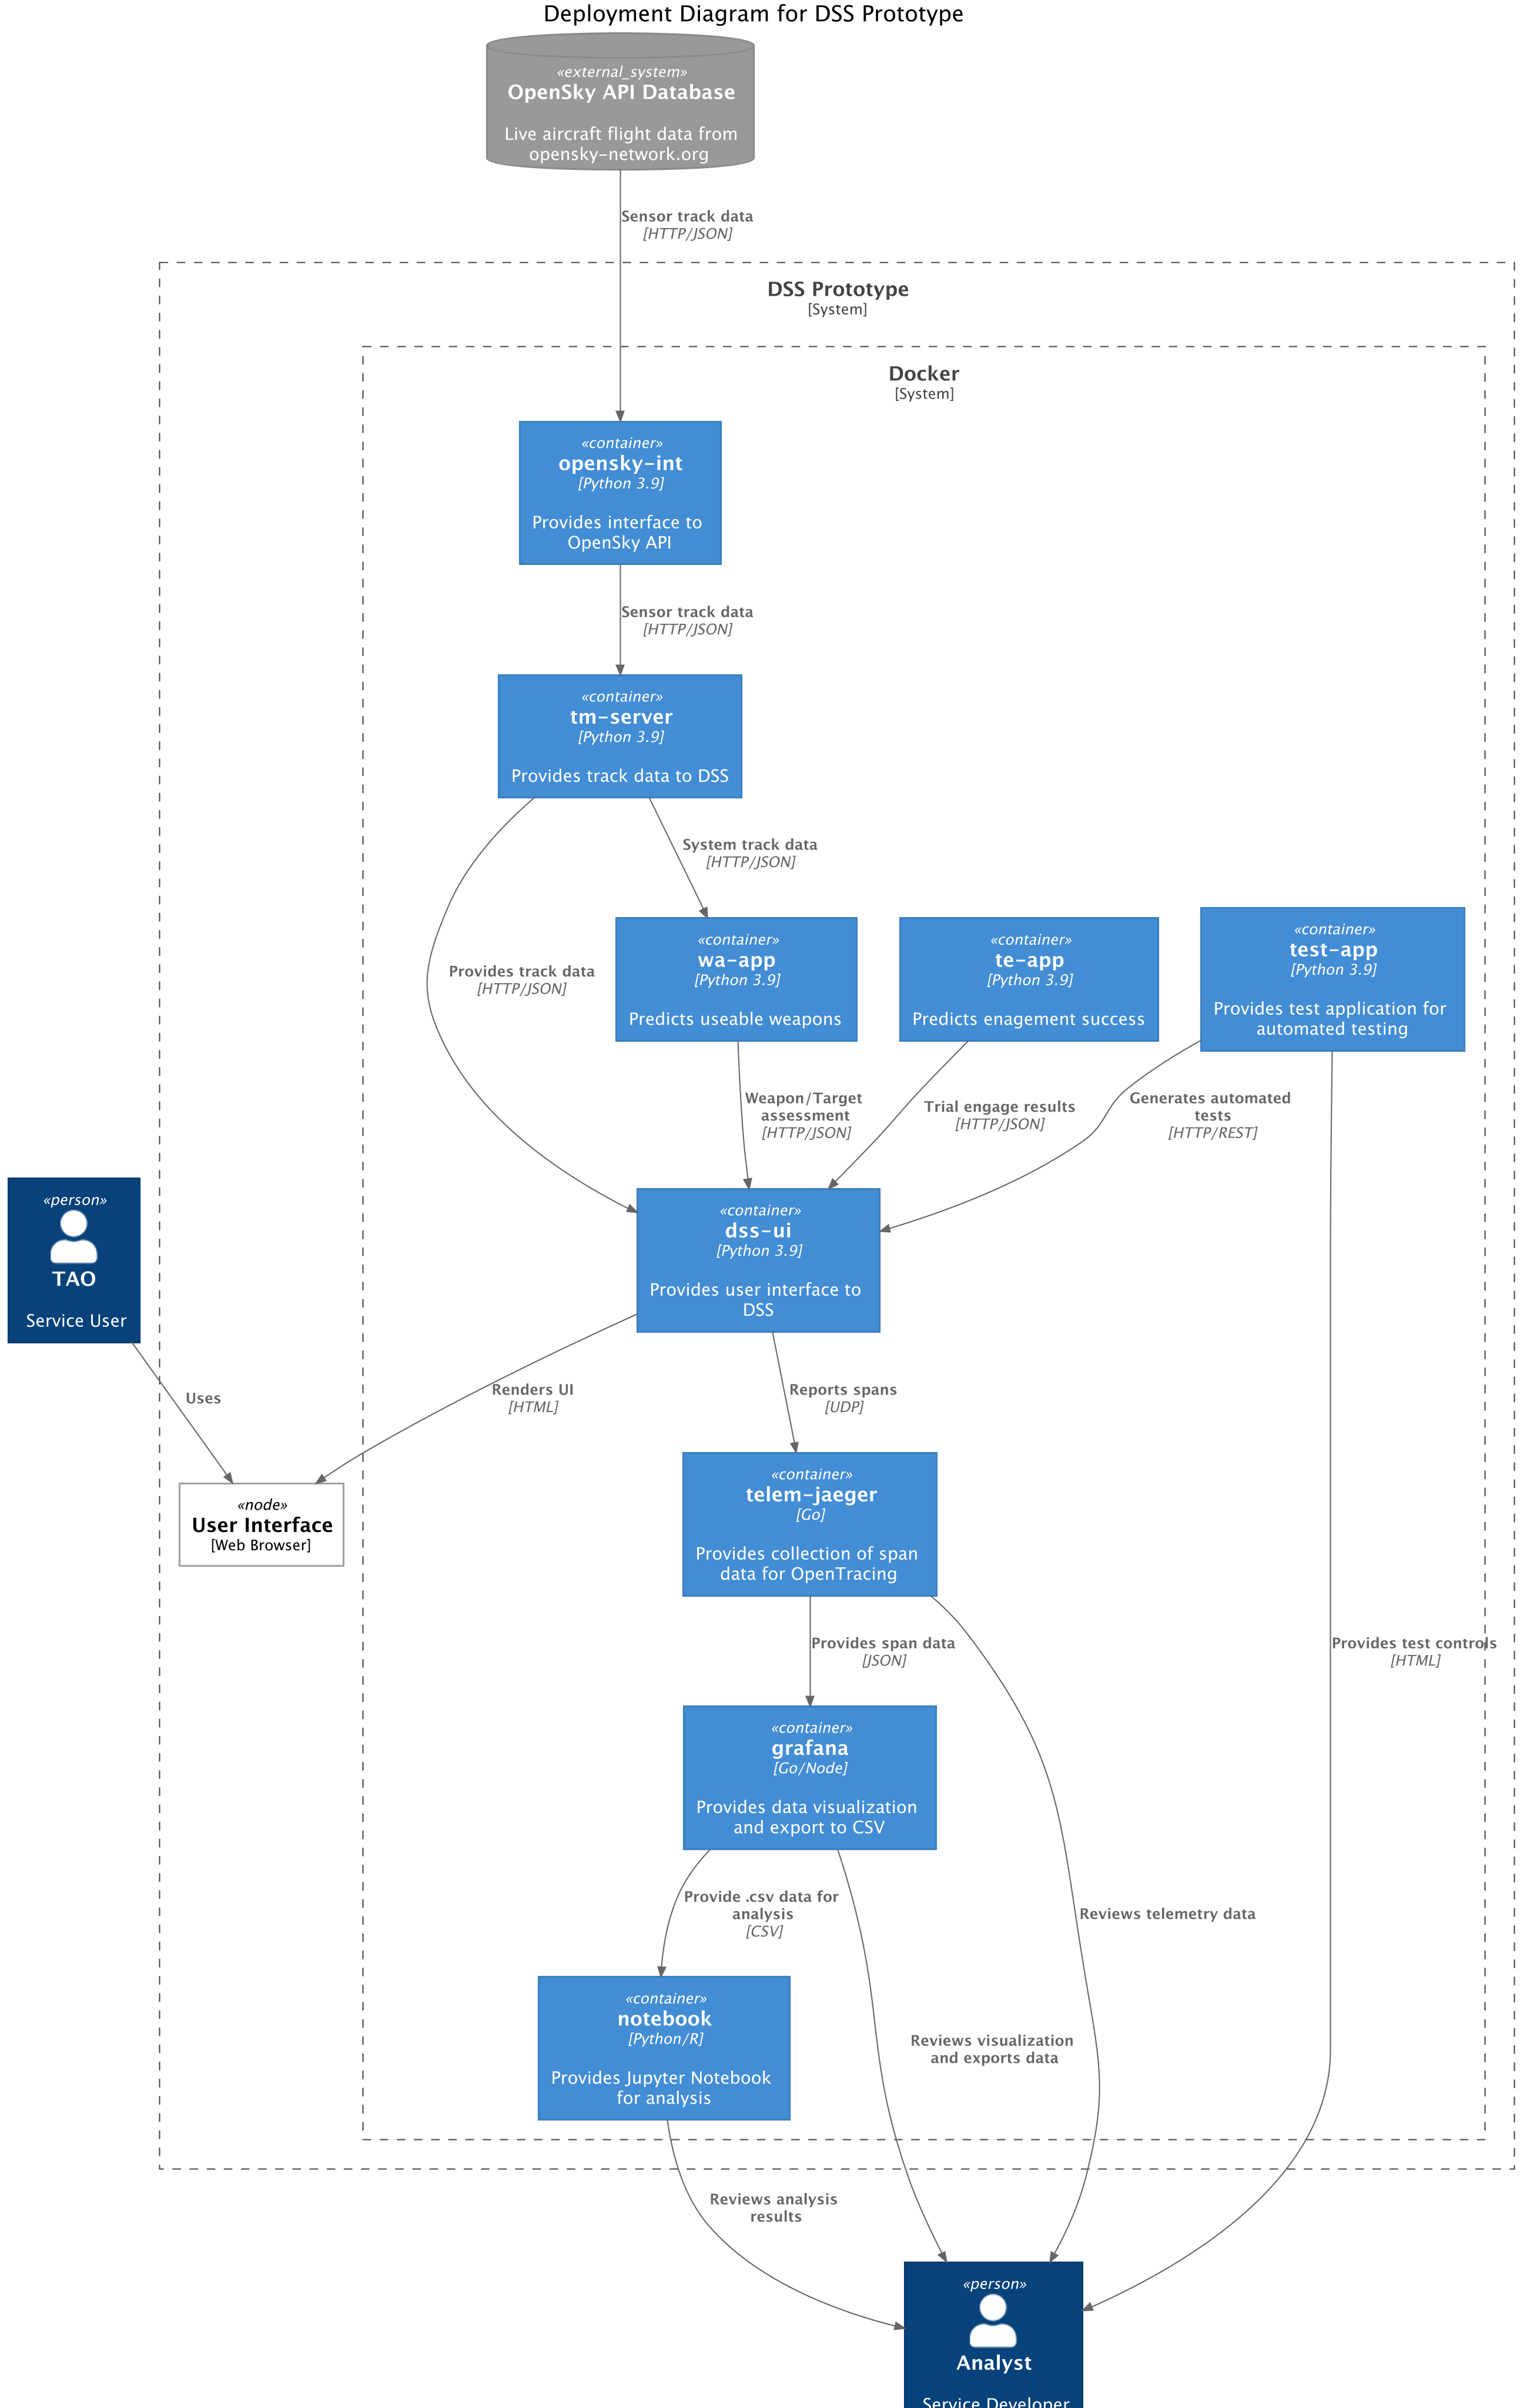
\includegraphics{dss-span-analysis-rev1_files/figure-pdf/fa6949b6-e2c7-4afc-89bd-057e476ef6cb.png}

}

\caption{DSS Deployment Diagram}

\end{figure}

\hypertarget{dss-applications}{%
\subsubsection{DSS Applications}\label{dss-applications}}

\begin{itemize}
\tightlist
\item
  opensky-int: Provides the OpenSky API for flight data. The app
  provides data about aircraft within 60 NM of Richmond (RIC) or Dulles
  (IAD) airports.
\item
  tm-server: Provides sensor track data (e.g.~OpenSky) and system tracks
  to support DSS services. System tracks represent the system-wide
  common understanding of track object states used for decision support.
\item
  wa-app: The Weapon Assessment Application determines which weapons are
  capable to successfully engage a target. The wa-app uses the tm-server
  api to get track data.
\item
  te-app: The Trail Engage Application predicts the success probability
  of an engagement with a specific weapon target pairing. The predicted
  track kinematic data at engagement time is provided; therefore, the
  current track kinematics from the tm-server are not queried prior to
  providing a response.
\item
  test-app: Provides an ability to initiate automated tests. the
  test-app uses the dss-ui to call dss-ui endpoint to replicate operator
  interactions with the DSS Prototype.
\item
  dss-ui: Provides a simple graphical interface to launch DSS services.
\end{itemize}

\hypertarget{dss-tools}{%
\subsubsection{DSS Tools}\label{dss-tools}}

\begin{itemize}
\tightlist
\item
  telem-jaeger: The open source Jaeger containter collects ``span'' data
  from the DSS applications. Spans collect duration data for service
  calls amongst containers; e.g.~latency. This the fundamental data that
  is being analysed here.
\item
  grafana: The open source Grafana container connects to the
  telem-jaeger container to create visualization dashboards. Also,
  Grafana faciliates the export of data as a .csv file for analysis.
\item
  notebook: The Jupyter Notebook container supports analysis of the data
  recorded by Jaeger and exported by Grafana. An embedded R software
  library is used for analysis.
\end{itemize}

\hypertarget{hypothesis}{%
\subsection{Hypothesis}\label{hypothesis}}

Hypotheses are ``innocent until proven guilty.'' We'll assume that
SpaceX and others have proven that DevSecOps tech can meet
hard-real-time requirements but nothing available in the body of
knowledge documents this.

\textbf{Hypothesis:} Modern DevSecOps architectures can be designed to
meet hard-real-time latency (\(\mu\)) requirements using modern
computing environments and computing infrastructure.

\(H_0: \mu \le 500 ms\) with jitter within latency bounds\\
\(H_a: \mu > 500 ms\) with jitter exceeding latency bounds

\emph{Murphy, Alvin C. and Moreland Jr, James D. `Integrating AI
Microservices into Hard-Real-Time SoS to Ensure Trustworthiness of
Digital Enterprise Using Mission Engineering'. 1 Jan.~2021 : 38 -- 54.}

\hypertarget{exploratory-data-analysis}{%
\section{Exploratory Data Analysis}\label{exploratory-data-analysis}}

\begin{verbatim}
   Trace.ID          Trace.name         Start.time          Duration        
 Length:100         Length:100         Length:100         Length:100        
 Class :character   Class :character   Class :character   Class :character  
 Mode  :character   Mode  :character   Mode  :character   Mode  :character  
\end{verbatim}

A data.frame: 6 × 2

\begin{longtable}[]{@{}lll@{}}
\toprule()
& Trace.ID \textless chr\textgreater{} & Trace.name
\textless chr\textgreater{} \\
\midrule()
\endhead
1 & 9ee3577fb1b427bc4fc17fecc5154d7d & dss-prototype: /TE \\
2 & f05ddc4dc13aff5c3098011b2a402401 & dss-prototype: /tracks \\
3 & 2bd901fbbfc9ee8dfa7c9629d93a1567 & dss-prototype: /IAD \\
4 & 69a48381a14e79da08aaa2353f7db4b2 & dss-prototype: /RIC \\
5 & e83037dcb9438c04dc12fba373b5502f & dss-prototype: /WA \\
6 & 7e381cd880adb670bb9627ca47020938 & dss-prototype: /TE \\
\bottomrule()
\end{longtable}

A data.frame: 6 × 2

\begin{longtable}[]{@{}lll@{}}
\toprule()
& Start.time \textless chr\textgreater{} & Duration
\textless chr\textgreater{} \\
\midrule()
\endhead
1 & 2022-05-02 10:25:01.366 & 36.0 ms \\
2 & 2022-05-02 10:25:00.309 & 43.3 ms \\
3 & 2022-05-02 10:24:58.818 & 464 ms \\
4 & 2022-05-02 10:24:57.307 & 494 ms \\
5 & 2022-05-02 10:24:56.128 & 139 ms \\
6 & 2022-05-02 10:24:55.081 & 30.3 ms \\
\bottomrule()
\end{longtable}

\hypertarget{convert-data-into-useable-metrics}{%
\subsection{Convert Data into Useable
Metrics}\label{convert-data-into-useable-metrics}}

To make the data more usable and easier to understand we apply
conversions from text to numeric and add additional columns with
supporting information. A \textbf{useCase} column is added to identify
specific DSS request use cases; e.g.~Get Dulles Airport Data. The data
also indicates whether the request is managed internally or a connection
to an external service is required to provided a response (i.e.,
https://opensky-network.org). A \textbf{numContainers} column is added
to indicate the number of containers involved in providing a use case
response (e.g.~independent variable). An \textbf{extNetworkHops} column
is added to include network hops for external requests as an additional
independent variable.

\begin{verbatim}
   Trace.ID          Trace.name          Start.time           Duration      
 Length:100         Length:100         Min.   :1.651e+09   Min.   :0.01390  
 Class :character   Class :character   1st Qu.:1.651e+09   1st Qu.:0.03275  
 Mode  :character   Mode  :character   Median :1.651e+09   Median :0.07375  
                                       Mean   :1.651e+09   Mean   :0.25404  
                                       3rd Qu.:1.651e+09   3rd Qu.:0.48450  
                                       Max.   :1.651e+09   Max.   :2.00000  
   useCase          numContainers extNetworkHops
 Length:100         Min.   :2.0   Min.   : 0.0  
 Class :character   1st Qu.:2.0   1st Qu.: 0.0  
 Mode  :character   Median :3.0   Median : 0.0  
                    Mean   :2.6   Mean   : 5.6  
                    3rd Qu.:3.0   3rd Qu.:14.0  
                    Max.   :3.0   Max.   :14.0  
\end{verbatim}

A data.frame: 6 × 3

\begin{longtable}[]{@{}
  >{\raggedright\arraybackslash}p{(\columnwidth - 6\tabcolsep) * \real{0.2500}}
  >{\raggedright\arraybackslash}p{(\columnwidth - 6\tabcolsep) * \real{0.2500}}
  >{\raggedright\arraybackslash}p{(\columnwidth - 6\tabcolsep) * \real{0.2500}}
  >{\raggedright\arraybackslash}p{(\columnwidth - 6\tabcolsep) * \real{0.2500}}@{}}
\toprule()
\begin{minipage}[b]{\linewidth}\raggedright
\end{minipage} & \begin{minipage}[b]{\linewidth}\raggedright
Trace.ID \textless chr\textgreater{}
\end{minipage} & \begin{minipage}[b]{\linewidth}\raggedright
Trace.name \textless chr\textgreater{}
\end{minipage} & \begin{minipage}[b]{\linewidth}\raggedright
Start.time \textless dbl\textgreater{}
\end{minipage} \\
\midrule()
\endhead
1 & 9ee3 & /TE & 1651487101 \\
2 & f05d & /tracks & 1651487100 \\
3 & 2bd9 & /IAD & 1651487098 \\
4 & 69a4 & /RIC & 1651487097 \\
5 & e830 & /WA & 1651487096 \\
6 & 7e38 & /TE & 1651487095 \\
\bottomrule()
\end{longtable}

A data.frame: 6 × 4

\begin{longtable}[]{@{}
  >{\raggedright\arraybackslash}p{(\columnwidth - 8\tabcolsep) * \real{0.2000}}
  >{\raggedright\arraybackslash}p{(\columnwidth - 8\tabcolsep) * \real{0.2000}}
  >{\raggedright\arraybackslash}p{(\columnwidth - 8\tabcolsep) * \real{0.2000}}
  >{\raggedright\arraybackslash}p{(\columnwidth - 8\tabcolsep) * \real{0.2000}}
  >{\raggedright\arraybackslash}p{(\columnwidth - 8\tabcolsep) * \real{0.2000}}@{}}
\toprule()
\begin{minipage}[b]{\linewidth}\raggedright
\end{minipage} & \begin{minipage}[b]{\linewidth}\raggedright
Duration \textless dbl\textgreater{}
\end{minipage} & \begin{minipage}[b]{\linewidth}\raggedright
useCase \textless chr\textgreater{}
\end{minipage} & \begin{minipage}[b]{\linewidth}\raggedright
numContainers \textless dbl\textgreater{}
\end{minipage} & \begin{minipage}[b]{\linewidth}\raggedright
extNetworkHops \textless dbl\textgreater{}
\end{minipage} \\
\midrule()
\endhead
1 & 0.0360 & Trial Engage (Internal) & 2 & 0 \\
2 & 0.0433 & Get Stored Local DSS Tracks (Internal) & 2 & 0 \\
3 & 0.4640 & Get Dulles Airport Data (External) & 3 & 14 \\
4 & 0.4940 & Get Richmond Airport Data (External) & 3 & 14 \\
5 & 0.1390 & Assess Weapons (Internal) & 3 & 0 \\
6 & 0.0303 & Trial Engage (Internal) & 2 & 0 \\
\bottomrule()
\end{longtable}

\hypertarget{exploratory-analysis-plots}{%
\subsection{Exploratory Analysis
Plots}\label{exploratory-analysis-plots}}

\begin{verbatim}
ERROR: Error in select(., Duration, numContainers, extNetworkHops): unused arguments (Duration, numContainers, extNetworkHops)
\end{verbatim}

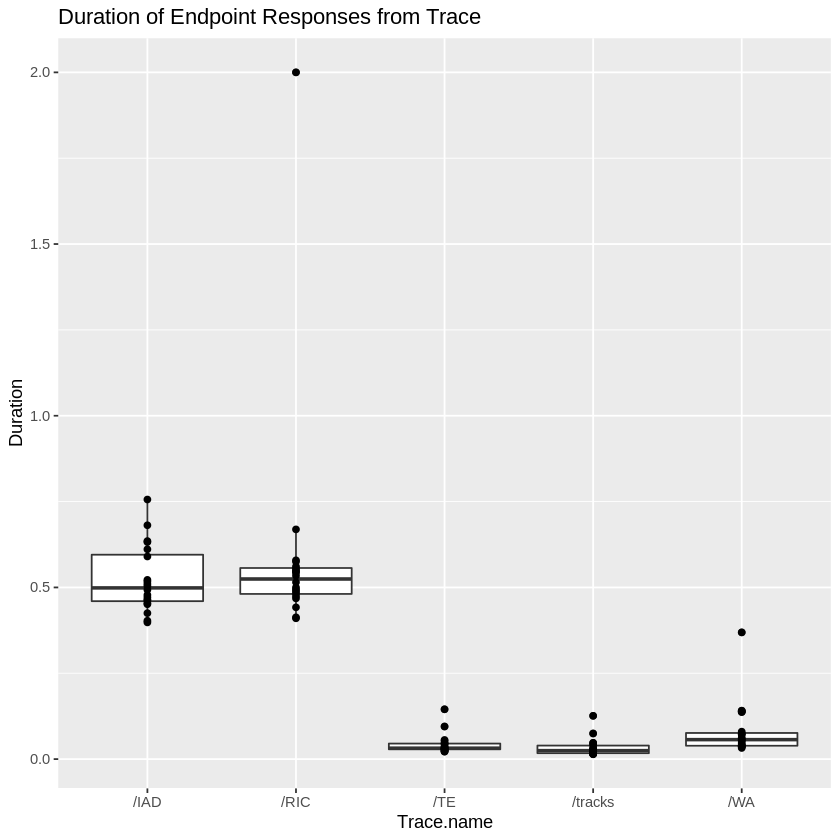
\includegraphics{dss-span-analysis-rev1_files/figure-pdf/cell-12-output-1.png}

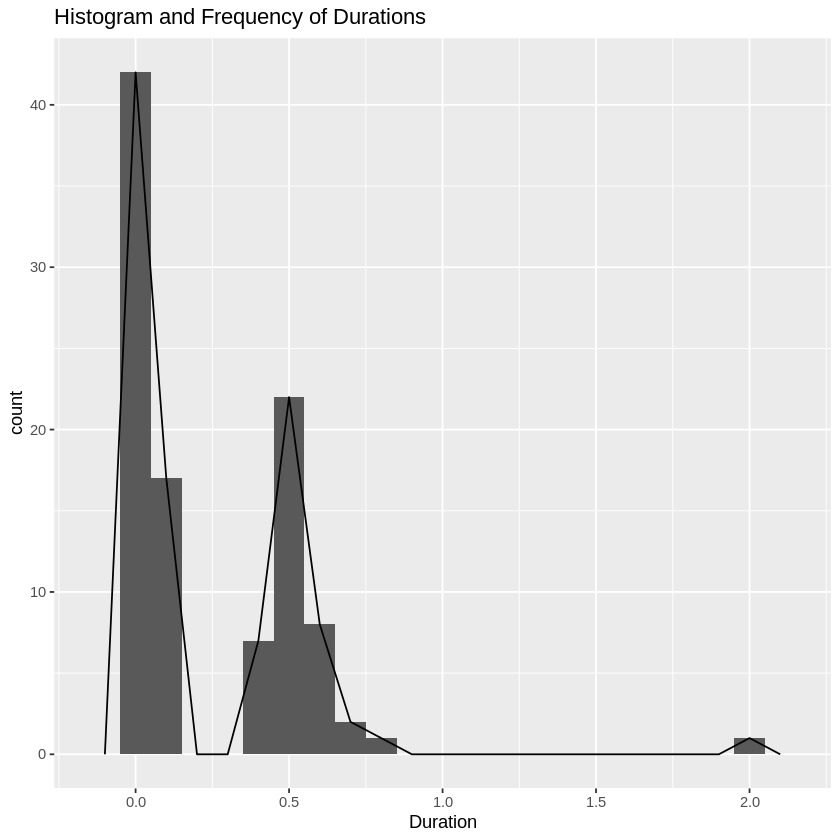
\includegraphics{dss-span-analysis-rev1_files/figure-pdf/cell-13-output-1.png}

\hypertarget{q-q-normality-test}{%
\subsection{Q-Q Normality Test}\label{q-q-normality-test}}

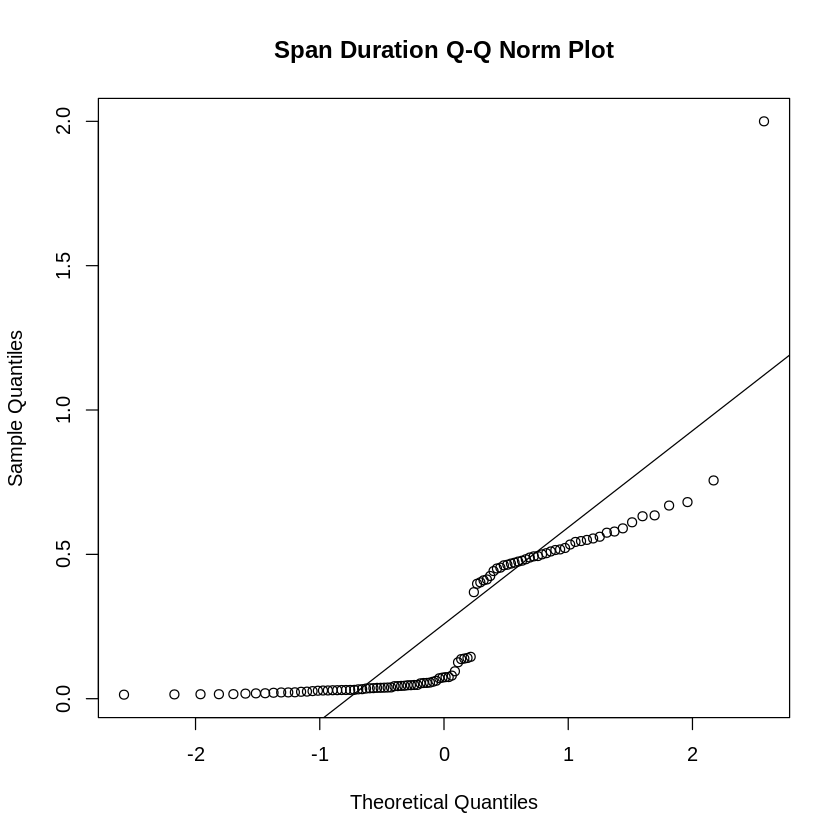
\includegraphics{dss-span-analysis-rev1_files/figure-pdf/cell-14-output-1.png}

A transformation is needed to apply statistical analysis.

\hypertarget{clean-the-data}{%
\section{Clean the Data}\label{clean-the-data}}

\hypertarget{search-for-outliers}{%
\subsection{Search for Outliers}\label{search-for-outliers}}

2

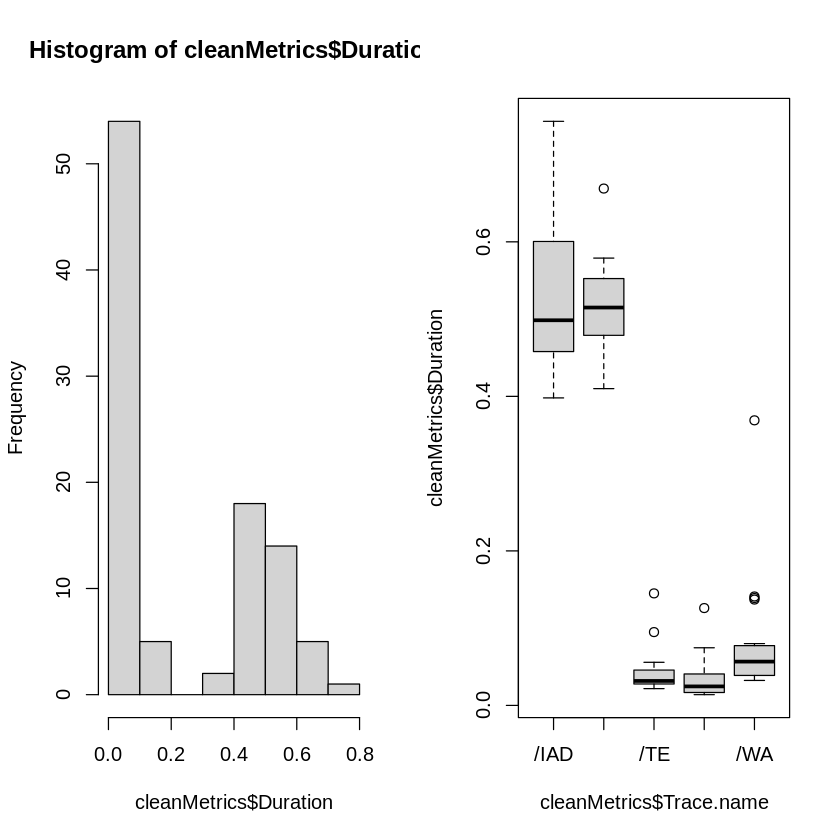
\includegraphics{dss-span-analysis-rev1_files/figure-pdf/cell-16-output-1.png}

\hypertarget{transformation-of-clean-metrics}{%
\subsection{Transformation of Clean
Metrics}\label{transformation-of-clean-metrics}}

\hypertarget{sqrt-log-and-cube-transformations}{%
\subsubsection{Sqrt, Log, and Cube
Transformations}\label{sqrt-log-and-cube-transformations}}

None of these transformation yield distributions that would be
considered normal. Most likely due to access to external and internal
services with differing latency. Lets try another transformation.

\hypertarget{box-cox-transformation}{%
\subsubsection{Box-Cox Transformation}\label{box-cox-transformation}}

Box and Cox (1964) developed a family of transformations designed to
reduce nonnormality of the errors in a linear model. Applying this
transform often reduces non-linearity as well, and heteroscedascity.

The idea is to transform the response variable \(Y\) to a replacement
response variable \(Y_i^{(\lambda)}\), leaving the right-hand side of
the regression model unchanged, so that the regression residuals become
normally-distributed. Note that the regression coefficients will also
change, because the response variable has changed; therefore, the
regression coefficients must be interpreted with respect to the
transformed variable. Also, any predictions made with the model have to
be back-transformed, to be interpreted in the original units.

The standard (simple) Box-Cox transform is:

\[
    Y_i^{(\lambda)}=
\begin{cases}
{\frac {Y_i^\lambda - 1} \lambda},  & {(\lambda \neq 0)} \\
log(Y_i), & {(\lambda = 0)}
\end{cases}
\]

\emph{Box, G. E. P., \& Cox, D. R. (1964). An Analysis of
Transformations. Journal of the Royal Statistical Society, Series B
(Metholodogical), 26(2), 211-252.}

http://www.css.cornell.edu/faculty/dgr2/\_static/files/R\_html/Transformations.html

\hypertarget{normality-testing-of-the-trasformation}{%
\subsection{Normality Testing of the
Trasformation}\label{normality-testing-of-the-trasformation}}

\hypertarget{shapiro-wilk}{%
\subsubsection{Shapiro-Wilk}\label{shapiro-wilk}}

The null-hypothesis of this test is that the population is normally
distributed. Thus, if the p value is less than the chosen alpha level,
then the null hypothesis is rejected and there is evidence that the data
tested are not normally distributed. On the other hand, if the p value
is greater than the chosen alpha level, then the null hypothesis (that
the data came from a normally distributed population) can not be
rejected (e.g., for an alpha level of .05, a data set with a p value of
less than .05 rejects the null hypothesis that the data are from a
normally distributed population).

https://en.wikipedia.org/wiki/Shapiro--Wilk\_test

With p-value of 2.852e-08 \textless{} 0.05 we reject the null hypothesis
that the data are from a normally distributed population. But we'll also
do a Q-Q Norm plot to visually see the results.

\emph{``if the p value is greater than the chosen alpha level, then the
null hypothesis (that the data came from a normally distributed
population) can not be rejected''}

\hypertarget{q-q-norm}{%
\subsubsection{Q-Q Norm}\label{q-q-norm}}

Our assumption here is that the separation of \textbf{Sample Quantiles}
is from the difference between internal and external span durations
(e.g.~latency). Let's see what happens when we split the samples.

\hypertarget{separating-original-internal-from-external-data}{%
\section{Separating ``Original'' Internal from External
Data}\label{separating-original-internal-from-external-data}}

\hypertarget{internal-data}{%
\subsection{Internal Data}\label{internal-data}}

This result looks much better. However, we'll remove internal span
outliers.

\hypertarget{q-q-norm-plot-of-clean-internal-span-data}{%
\subsubsection{Q-Q Norm Plot of ``Clean'' Internal Span
Data}\label{q-q-norm-plot-of-clean-internal-span-data}}

We'll look a the Q-Q Norm Plot and Shapiro-Wilk Test

\hypertarget{autocorrelation}{%
\subsubsection{Autocorrelation}\label{autocorrelation}}

Autocorrelation plots are a commonly-used tool for checking randomness
in a data set. This randomness is ascertained by computing
autocorrelations for data values at varying time lags. If random, such
autocorrelations should be near zero for any and all time-lag
separations. If non-random, then one or more of the autocorrelations
will be significantly non-zero.

\hypertarget{shapiro-wilk-normality-test}{%
\subsubsection{Shapiro-Wilk Normality
Test}\label{shapiro-wilk-normality-test}}

With p-value of 0.002321 \textless{} 0.05 we reject the null hypothesis
that the data are from a normally distributed population.

\emph{``if the p value is greater than the chosen alpha level, then the
null hypothesis (that the data came from a normally distributed
population) can not be rejected''}

\hypertarget{data-transformations}{%
\subsubsection{Data Transformations}\label{data-transformations}}

\hypertarget{sqrt-log-cube-transformations}{%
\paragraph{Sqrt-Log-Cube
Transformations}\label{sqrt-log-cube-transformations}}

\hypertarget{q-q-norm-sqrt-log-cube}{%
\paragraph{Q-Q Norm Sqrt-Log-Cube}\label{q-q-norm-sqrt-log-cube}}

\hypertarget{shapiro-wilk-testing-sqrt-log-cube}{%
\paragraph{Shapiro-Wilk Testing
Sqrt-Log-Cube}\label{shapiro-wilk-testing-sqrt-log-cube}}

The \textbf{cube transformation} seems to provide the best q-q plot fit.
With a p-value of 0.3593 \textgreater{} 0.05 we fail to reject the null
hypothesis and assume we now have a normal distribution.

\emph{``if the p value is greater than the chosen alpha level, then the
null hypothesis (that the data came from a normally distributed
population) can not be rejected''}

\hypertarget{autocorrelation-1}{%
\subsubsection{Autocorrelation}\label{autocorrelation-1}}

Autocorrelation plots are a commonly-used tool for checking randomness
in a data set. This randomness is ascertained by computing
autocorrelations for data values at varying time lags. If random, such
autocorrelations should be near zero for any and all time-lag
separations. If non-random, then one or more of the autocorrelations
will be significantly non-zero.

The ACF indicates that the data is random since the results are near
zero.

\hypertarget{hypothesis-testing}{%
\subsubsection{Hypothesis Testing}\label{hypothesis-testing}}

We will use a Student's t-Test to test the hypothesis on \textbf{normal}
internal span data. Our mean is 500 ms (e.g.~\(\mu = 0.5\) seconds) and
our null hypthesis is less than 500 ms.

With a original and transformation with a p-value of 1 \textgreater{}
0.05 we fail to reject the null hypothesis, i.e.~we assume that latency
will be less than 500 ms.

\emph{``If the p value is greater than the chosen alpha level, then the
null hypothesis (that latency is \textless{} 500 ms) can not be
rejected''}

\hypertarget{external-data}{%
\subsection{External Data}\label{external-data}}

\hypertarget{q-q-norm-plot-of-clean-external-span-data}{%
\subsubsection{Q-Q Norm Plot of ``Clean'' External Span
Data}\label{q-q-norm-plot-of-clean-external-span-data}}

We'll look a the Q-Q Norm Plot and Shapiro-Wilk Test

\hypertarget{shapiro-wilk-normality-test-1}{%
\subsubsection{Shapiro-Wilk Normality
Test}\label{shapiro-wilk-normality-test-1}}

With a p-value of 0.2878 \textgreater{} 0.05 we fail to reject the null
hypothesis, i.e.~we assume that we have a normal distribution.

\hypertarget{autocorrelation-2}{%
\subsubsection{Autocorrelation}\label{autocorrelation-2}}

The ACF indicates that the data is random since the results are near
zero.

\hypertarget{hypothesis-testing-1}{%
\subsubsection{Hypothesis Testing}\label{hypothesis-testing-1}}

We will use a Student's t-Test to test the hypothesis on external span
data. Our mean is 500 ms (e.g.~\(\mu = 0.5\) seconds) and our null
hypthesis is less than 500 ms.

With a p-value of 0.1336 \textgreater{} 0.05 we fail to reject the null
hypothesis, i.e.~we assume that 500 ms can be maintained for external
service requests.

\emph{``If the p value is greater than the chosen alpha level, then the
null hypothesis (that latency is \textless{} 500 ms) can not be
rejected''}

\hypertarget{observations}{%
\section{Observations}\label{observations}}

\hypertarget{general-discussion-of-normality}{%
\subsection{General Discussion of
Normality}\label{general-discussion-of-normality}}

It was required to separate external data from internal to establish
normality of the data samples. The internal data set required
transformation to establish normality, while the external data did not
require a transformation.

\hypertarget{hypothesis-results}{%
\subsection{Hypothesis Results}\label{hypothesis-results}}

Hypothesis testing using the Student's t-Test indicates that latency
constraints of 500 ms can be maintained internally and external.
However, serveral external samples were greater than 500 ms. This is
most likely due to the non-deterministic nature of internet (e.g.~http)
requests. Within the internal environment, data is directly routed
between microservices within the Docker environment within a private
network. The data shows that a container based microservice architecture
can meet the requirement; however, care must be taken to manage
processing per container that may increase container response times.



\end{document}
